\chapter{Implementation}
Marty is written in Python and PL/pgSQL with a small patch to the Postgres source code written in C.
Python and PL/pgSQL are both high-level programming languages and ideal for rapid prototyping.
The source code cointains two scripts, \textit{clone.py} and \textit{history.py}, which are used to create and populate the clone databases and the history database, respectively.
The patch to Postgres is necessary for Marty to be able to read the changes from the write-ahead log (WAL) with the slave instance.

Marty is designed to work with Postgres 9.3.3.
The patch is written for this version and might not work with other versions, older or newer.

This chapter describes the implementation of Marty.
It explains which parts of Postgres Marty uses to create the history database and keep track of the changes that are made to the master database.
It starts by explaining how the slave instance is used and why it is patched.
It then continues with a description of the history database and its design and ends with a description of the clone databases and how they use the history database to imitate the master.

\section{The slave instance}

\begin{wrapfigure}{r}{0.4\textwidth}
  \vspace{-20pt}
  \begin{center}
    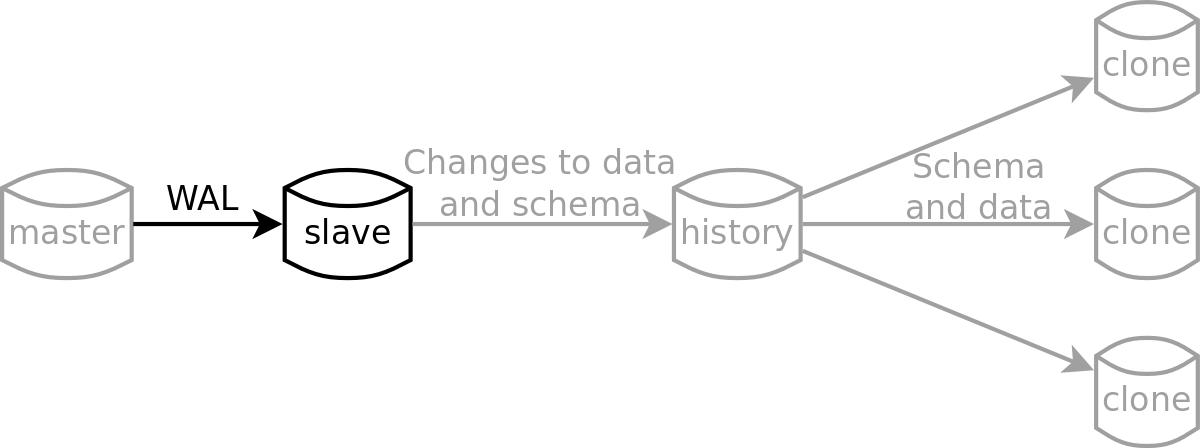
\includegraphics[width=0.38\textwidth]{img/architecture-slave}
  \end{center}
  \vspace{-20pt}
  \caption{The slave part of the architecture}
  \vspace{-10pt}
\end{wrapfigure}

Marty uses the slave instance to initialize the history database and to inspect the contents of the WAL from the master.
The slave is configured to act as a \textit{hot standby} for the master; it starts with a copy of the master database and updates it with the WAL from the master.
A hot standby can be queried with read only quries and when the slave database is first started Marty copies its schema and data to the history database.
It then inspects the changes from the WAL as they are applied and updates the history database accordingly.

Before the slave instance is started the database administrator that manages the master must configure it correctly.
This includes configuring a few parameters in the \textit{postgres.conf} file, see table \ref{table:master-config}.
Next the administrator must take a \textit{base-backup} of the master database.
This can be done with the program \textit{pg\_basebackup} and might require changes to the \textit{pg\_hba.conf} file, see the Postgres documentation for further reference. % TODO add referernce?

\begin{table}[h]
  \centering
  \texttt{
    \begin{tabular}{| l | l |}
      \hline
      \textbf{Parameter} & \textbf{Value} \\ \hline
      wal\_level & hot\_standby \\ \hline
      archive\_mode & on \\ \hline
      archive\_command & 'cp \%p /path/to/archive/\%f' \\ \hline
      max\_wal\_senders & 1 \\ \hline
    \end{tabular}
  }
  \caption{Configuration parameters in postgres.conf for the master database}
  \medskip
  \small
  This archive command is just an example, when the master is configured it must use an archive command that copies the WAL files to a storage where they are accessible by the slave.
  Also note that \texttt{max\_wal\_senders} must at least be 1, but can be higher.
  \label{table:master-config}
\end{table}

As previously noted the slave runs on a patched version of Postgres that must be compiled with a special flag that enables Postgres to log the WAL replay actions.
When the patch has been applied to the Postgres source code it must be compiled with the \texttt{WAL\_DEBUG} CPP flag.

Instead of creating a new cluster for the slave with the \texttt{initdb} command the administrator should use the files from the base-backup.
When they have been copied to the correct place the \textit{postgres.conf} file must be updated, see table \ref{table:slave-config}.
It is then necessary to add a \textit{recovery.conf} file with a command to fetch the WAL files from the master database, see the Postgres documentation for further reference. % TODO reference?

\begin{table}[h]
  \centering
  \texttt{
    \begin{tabular}{| l | l |}
      \hline
      \textbf{Parameter} & \textbf{Value} \\ \hline
      hot\_standby & on \\ \hline
      wal\_debug & on \\ \hline
    \end{tabular}
  }
  \caption{Configuration parameters in postgres.conf for the slave database}
  \label{table:slave-config}
\end{table}
\
